\documentclass{article}
\usepackage{tikz}

\begin{document}


\begin{center}
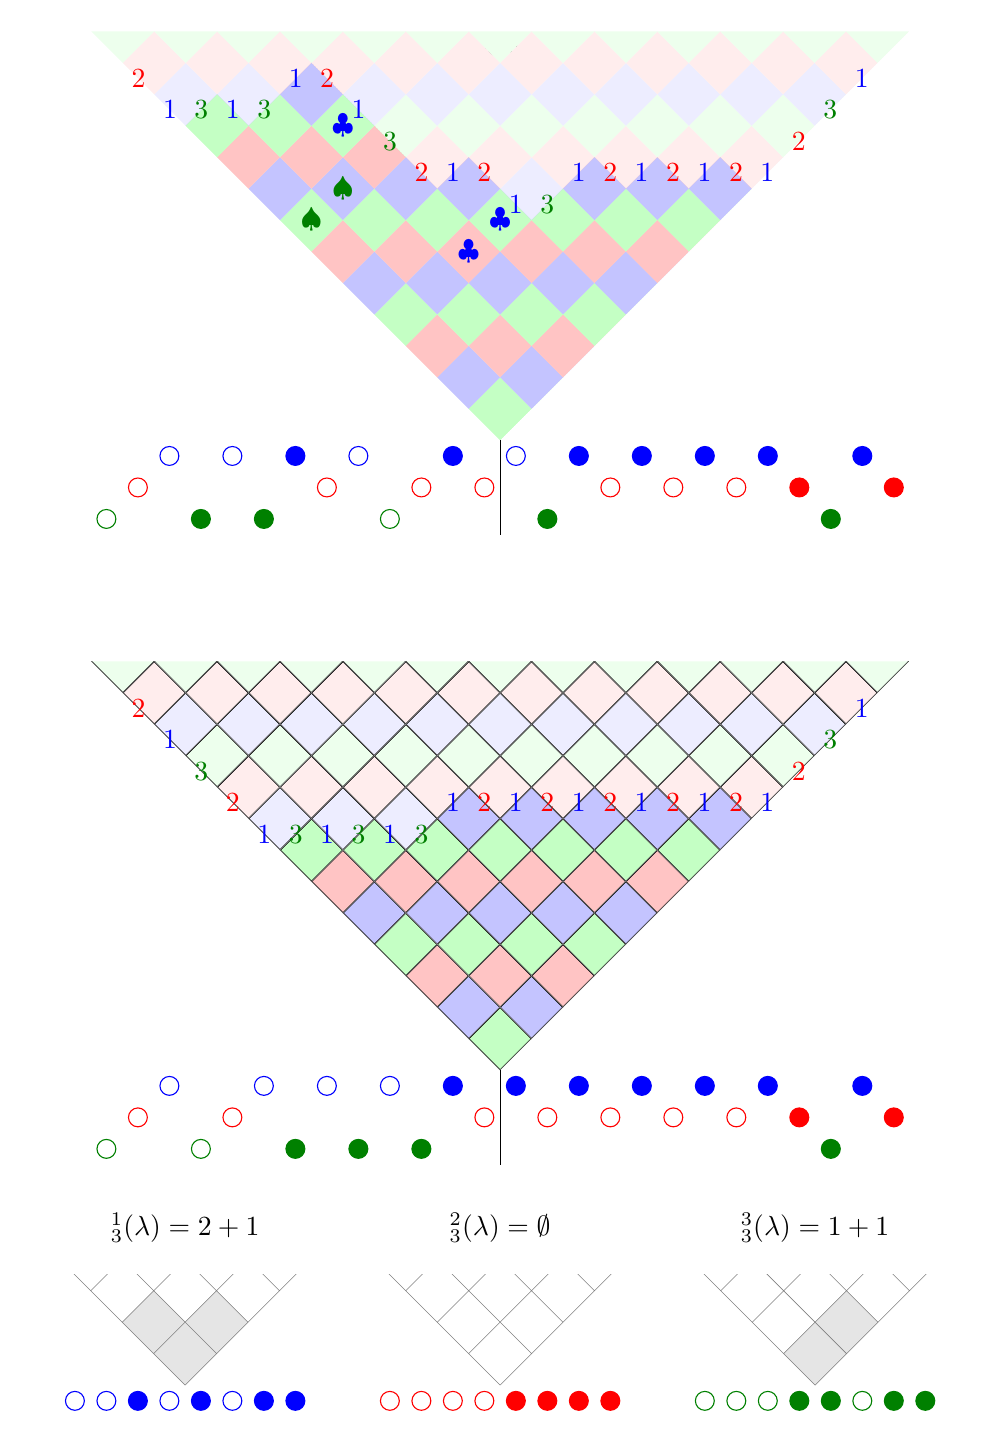
\begin{tikzpicture}

\begin{scope} %drawing of original partition
\draw (0,5) node{$\lambda=$};
\begin{scope}[scale=.4]

\begin{scope}[rotate=45, scale=1.412]
\clip (0,0)--(13,0)--(0,13)--(0,0);
\foreach \x in {0,...,13}{%
    \foreach \y in {0,...,4}{%
       \fill[green!7]  (\x, -\x+3*\y) rectangle (\x+1, -\x+3*\y+1); 
       \fill[blue!7]  (\x, -\x+3*\y+1) rectangle (\x+1, -\x+3*\y+2); 
       \fill[red!7]  (\x, -\x+3*\y+2) rectangle (\x+1, -\x+3*\y+3); 
}}
\end{scope}


\begin{scope}[rotate=45, scale=1.412]
\clip (0,0)--(0,10)--(1,10)--(1,9)--(3,9)--(3,5)--(4,5)--(4,3)--(6,3)--(6,2)--(7,2)--(7,1)--(8,1)--(8,0)--(0,0);
\foreach \x in {0,...,13}{%
    \foreach \y in {0,...,4}{%
       \fill[fill=green!23]  (\x, -\x+3*\y) rectangle (\x+1, -\x+3*\y+1); 
       \fill[fill=blue!23]  (\x, -\x+3*\y+1) rectangle (\x+1, -\x+3*\y+2); 
       \fill[fill=red!23]  (\x, -\x+3*\y+2) rectangle (\x+1, -\x+3*\y+3); 
}}
\end{scope}




      \begin{scope}[rotate=45, scale=1.412, black!50!green] 
         \draw (.5,6.5)node{$\spadesuit$};
         \draw (1.5,6.5)node{$\spadesuit$};
      \end{scope}

      \begin{scope}[rotate=45, scale=1.412, blue] 
         \draw (2.5,7.5)node{$\clubsuit$};
         \draw (2.5,3.5)node{$\clubsuit$};
         \draw (3.5,3.5)node{$\clubsuit$};
      \end{scope}



   \end{scope}

   \begin{scope}[rotate=45, ultra thick, scale=.4*1.412]
      \begin{scope}[blue]
         \draw (0,10.5) node{$1$};
         \draw (1,9.5)node{$1$};
         \draw (2.5,9)node{$1$};
         \draw (3,7.5)node{$1$};
         \draw (3.5,5)node{$1$};
         \draw (4,3.5)node{$1$};
         \draw (5.5,3)node{$1$};
         \draw (6.5,2)node{$1$};
         \draw (7.5,1)node{$1$};
         \draw (8.5,0)node{$1$};
         \draw (11.5,0)node{$1$};
      \end{scope}

      \begin{scope}[red]
         \draw (0,11.5)node{$2$};
         \draw (3,8.5)node{$2$};
         \draw (3,5.5)node{$2$};
         \draw (4,4.5)node{$2$};
         \draw (6,2.5)node{$2$};
         \draw (7,1.5)node{$2$};
         \draw (8,.5)node{$2$};
         \draw (9.5,0)node{$2$};
      \end{scope}

      \begin{scope}[black!50!green]
         \draw (.5,10)node{$3$};
         \draw (1.5, 9)node{$3$};
         \draw (3,6.5)node{$3$};
         \draw (4.5,3)node{$3$};
         \draw (10.5,0)node{$3$};

      \end{scope}

   \end{scope}

   \begin{scope}[scale=.4, yshift=-.5cm, blue]
      \draw(-10.5,0) circle(.3);
      \draw(-8.5, 0)  circle (.3);
      \filldraw(-6.5,0)  circle (.3);
      \draw(-4.5,0)  circle (.3);
      \filldraw(-1.5,0)  circle (.3);
      \draw(.5,0)  circle (.3);
      \filldraw(2.5,0)  circle (.3);
      \filldraw(4.5,0)  circle (.3);
      \filldraw(6.5,0)  circle (.3);
      \filldraw(8.5,0)  circle (.3);
      \filldraw(11.5,0)  circle (.3);
   \end{scope}

   \begin{scope}[scale=.4, yshift=-1.5cm, red]
      \draw(-11.5,0) circle(.3);
      \draw(-5.5, 0)  circle (.3);
      \draw(-2.5,0)  circle (.3);
      \draw(-.5,0)  circle (.3);
      \draw(3.5,0)  circle (.3);
      \draw(5.5,0)  circle (.3);
      \draw(7.5,0)  circle (.3);
      \filldraw(9.5,0)  circle (.3);
      \filldraw(12.5,0)  circle (.3);
   \end{scope}

   \begin{scope}[scale=.4, yshift=-2.5cm, black!50!green]
      \draw(-12.5,0)  circle (.3);
      \filldraw(-9.5,0) circle(.3);
      \filldraw(-7.5, 0)  circle (.3);
      \draw(-3.5,0)  circle (.3);
      \filldraw(1.5,0)  circle (.3);
      \filldraw(10.5,0)  circle (.3);
   \end{scope}

   \begin{scope}[scale=.4]
      \draw (0,-3)--(0,0);
   \end{scope}
\end{scope}

\begin{scope}[yshift=-8cm] %drawing of the core
\draw (0,5) node{$\core_3(\lambda)=7+5+3+3+2+2+1+1$};



\begin{scope}[rotate=45, scale=.4*1.412]

\clip (0,0)--(13,0)--(0,13)--cycle;
\foreach \x in {0,...,13}{%
    \foreach \y in {0,...,4}{%
       \draw[fill=green!7]  (\x, -\x+3*\y) rectangle (\x+1, -\x+3*\y+1); 
       \draw[fill=blue!7]  (\x, -\x+3*\y+1) rectangle (\x+1, -\x+3*\y+2); 
       \draw[fill=red!7]  (\x, -\x+3*\y+2) rectangle (\x+1, -\x+3*\y+3); 
}}

\begin{scope}
    \clip (0,0)--(0,7)--(1,7)--(1,6)--(2,6)--(2,5)--(4,5)--(4,4)--(5,4)--(5,3)--(6,3)--(6,2)--(7,2)--(7,1)--(8,1)--(8,0)--cycle;
\foreach \x in {0,...,13}{%
    \foreach \y in {0,...,4}{%
       \draw[fill=green!23]  (\x, -\x+3*\y) rectangle (\x+1, -\x+3*\y+1); 
       \draw[fill=blue!23]  (\x, -\x+3*\y+1) rectangle (\x+1, -\x+3*\y+2); 
       \draw[fill=red!23]  (\x, -\x+3*\y+2) rectangle (\x+1, -\x+3*\y+3); 
}}
\end{scope}


      \draw[gray, very thin] (0,0) grid (13,13);
\end{scope}


   \begin{scope}[rotate=45, ultra thick, scale=.4*1.412]
      \begin{scope}[blue]
         \draw (0,10.5) node{$1$};
         \draw (0,7.5)node{$1$};
         \draw (1,6.5)node{$1$};
         \draw (2,5.5)node{$1$};
         \draw (3.5,5)node{$1$};
         \draw (4.5,4)node{$1$};
         \draw (5.5,3)node{$1$};
         \draw (6.5,2)node{$1$};
         \filldraw (7.5,1)node{$1$};
         \filldraw (8.5,0)node{$1$};
         \filldraw (11.5,0)node{$1$};
      \end{scope}

      \begin{scope}[red]
         \draw (0,11.5)node{$2$};
         \draw (0,8.5)node{$2$};
         \draw (4, 4.5)node{$2$};
         \draw (5, 3.5)node{$2$};
         \draw (6, 2.5)node{$2$};
         \draw (7, 1.5)node{$2$};
         \draw (8,.5)node{$2$};
         \draw (9.5,0)node{$2$};
      \end{scope}

      \begin{scope}[black!50!green]
         \draw (0,9.5)node{$3$};
         \draw (0.5, 7)node{$3$};
         \draw (1.5,6)node{$3$};
         \draw (2.5,5)node{$3$};
         \draw (10.5,0)node{$3$};
      \end{scope}

   \end{scope}

   \begin{scope}[scale=.4, yshift=-.5cm, blue]
      \draw(-10.5,0) circle(.3);
      \draw(-7.5, 0)  circle (.3);
      \draw(-5.5,0)  circle (.3);
      \draw(-3.5,0)  circle (.3);
      \filldraw(-1.5,0)  circle (.3);
      \filldraw(.5,0)  circle (.3);
      \filldraw(2.5,0)  circle (.3);
      \filldraw(4.5,0)  circle (.3);
      \filldraw(6.5,0)  circle (.3);
      \filldraw(8.5,0)  circle (.3);
      \filldraw(11.5,0)  circle (.3);
   \end{scope}

   \begin{scope}[scale=.4, yshift=-1.5cm, red]
      \draw(-11.5,0) circle(.3);
      \draw(-8.5, 0)  circle (.3);
      \draw(-.5,0)  circle (.3);
      \draw(1.5,0)  circle (.3);
      \draw(3.5,0)  circle (.3);
      \draw(5.5,0)  circle (.3);
      \draw(7.5,0)  circle (.3);
      \filldraw(9.5,0)  circle (.3);
      \filldraw(12.5,0)  circle (.3);
   \end{scope}

   \begin{scope}[scale=.4, yshift=-2.5cm, black!50!green]
          \draw(-12.5,0) circle(.3);
      \draw(-9.5,0) circle(.3);
      \filldraw(-6.5, 0)  circle (.3);
      \filldraw(-4.5,0)  circle (.3);
      \filldraw(-2.5,0)  circle (.3);
       \filldraw(10.5,0)  circle (.3);
   \end{scope}

   \begin{scope}[scale=.4]
      \draw (0,-3)--(0,0);
   \end{scope}

\end{scope}


\begin{scope}[yshift=-12cm] %the quotients

   \begin{scope}[xshift=-4cm] %blue quotient


\draw (0,2) node{$\quot_3^1(\lambda)=2+1$};
      \begin{scope}[gray, very thin, scale=.4]
         \clip (-5, 3.5) rectangle (5, -1);
         \draw[rotate=45, scale=1.412, gray!20!white, fill] (0,0)--(0,2)--(1,2)--(1,1)--(2,1)--(2,0)--cycle;
         \draw[rotate=45, scale=1.412] (0,0) grid (4,4);
      \end{scope}

      \begin{scope}[scale=.4, yshift=-.5cm, blue]
         \draw(-3.5,0) circle(.3);
         \draw(-2.5, 0)  circle (.3);
         \filldraw(-1.5,0)  circle (.3);
         \draw(-.5,0)  circle (.3);
         \filldraw(.5,0)  circle (.3);
         \draw(1.5,0)  circle (.3);
         \filldraw(2.5,0)  circle (.3);
         \filldraw(3.5,0)  circle (.3);
      \end{scope}

   \end{scope}



   \begin{scope} %red quotient
\draw (0,2) node{$\quot_3^2(\lambda)=\emptyset$};
      \begin{scope}[gray, very thin, scale=.4]
         \clip (-5, 3.5) rectangle (5, -1);
         \draw[rotate=45, scale=1.412] (0,0) grid (4,4);
      \end{scope}

      \begin{scope}[scale=.4, yshift=-.5cm, red]
         \draw(-3.5,0) circle(.3);
         \draw(-2.5, 0)  circle (.3);
         \draw(-1.5,0)  circle (.3);
         \draw(-.5,0)  circle (.3);
         \filldraw(.5,0)  circle (.3);
         \filldraw(1.5,0)  circle (.3);
         \filldraw(2.5,0)  circle (.3);
         \filldraw(3.5,0)  circle (.3);
      \end{scope}

   \end{scope}


   \begin{scope}[xshift=4cm] %green quotient 
\draw (0,2) node{$\quot_3^3(\lambda)=1+1$};

      \begin{scope}[gray, very thin, scale=.4]
         \clip (-5, 3.5) rectangle (5, -1);
         \draw[rotate=45, scale=1.412, gray!20!white, fill] (0,0)--(0,1)--(2,1)--(2,0)--cycle;
         \draw[rotate=45, scale=1.412] (0,0) grid (4,4);
      \end{scope}

      \begin{scope}[scale=.4, yshift=-.5cm, black!50!green]
         \draw(-3.5,0) circle(.3);
         \draw(-2.5, 0)  circle (.3);
         \draw(-1.5,0)  circle (.3);
         \filldraw(-.5,0)  circle (.3);
         \filldraw(.5,0)  circle (.3);
         \draw(1.5,0)  circle (.3);
         \filldraw(2.5,0)  circle (.3);
         \filldraw(3.5,0)  circle (.3);
      \end{scope}

   \end{scope}

\end{scope}


\end{tikzpicture}
\end{center}


\end{document}
